\section{thread.h File Reference}
\label{thread_8h}\index{thread.h@{thread.h}}
{\tt \#include \char`\"{}machine.h\char`\"{}}\par
{\tt \#include \char`\"{}memory.h\char`\"{}}\par
{\tt \#include \char`\"{}regs.h\char`\"{}}\par


Include dependency graph for thread.h:\nopagebreak
\begin{figure}[H]
\begin{center}
\leavevmode
\includegraphics[width=420pt]{thread_8h__incl}
\end{center}
\end{figure}


This graph shows which files directly or indirectly include this file:\nopagebreak
\begin{figure}[H]
\begin{center}
\leavevmode
\includegraphics[width=420pt]{thread_8h__dep__incl}
\end{center}
\end{figure}
\subsection*{Classes}
\begin{CompactItemize}
\item 
struct {\bf thread\_\-t}
\end{CompactItemize}
\subsection*{Defines}
\begin{CompactItemize}
\item 
\#define {\bf BOOT\_\-PC}~0x00000000
\end{CompactItemize}
\subsection*{Functions}
\begin{CompactItemize}
\item 
int {\bf sim\_\-load\_\-prog} (struct {\bf thread\_\-t} $\ast$thread, char $\ast$fname, int argc, char $\ast$$\ast$argv, char $\ast$$\ast$envp)
\item 
void {\bf sim\_\-aux\_\-config} (FILE $\ast$stream)
\item 
void {\bf sim\_\-aux\_\-stats} (FILE $\ast$stream)
\item 
void {\bf sim\_\-uninit} (void)
\end{CompactItemize}
\subsection*{Variables}
\begin{CompactItemize}
\item 
struct {\bf thread\_\-t} $\ast$$\ast$ {\bf threads}
\item 
unsigned int {\bf num\_\-threads}
\item 
int {\bf simulated\_\-processes\_\-remaining}
\end{CompactItemize}


\subsection{Define Documentation}
\index{thread.h@{thread.h}!BOOT\_\-PC@{BOOT\_\-PC}}
\index{BOOT\_\-PC@{BOOT\_\-PC}!thread.h@{thread.h}}
\subsubsection[{BOOT\_\-PC}]{\setlength{\rightskip}{0pt plus 5cm}\#define BOOT\_\-PC~0x00000000}\label{thread_8h_3e8bd7832d770102979335a24585c78f}




Definition at line 8 of file thread.h.

Referenced by sim\_\-post\_\-init().

\subsection{Function Documentation}
\index{thread.h@{thread.h}!sim\_\-aux\_\-config@{sim\_\-aux\_\-config}}
\index{sim\_\-aux\_\-config@{sim\_\-aux\_\-config}!thread.h@{thread.h}}
\subsubsection[{sim\_\-aux\_\-config}]{\setlength{\rightskip}{0pt plus 5cm}void sim\_\-aux\_\-config (FILE $\ast$ {\em stream})}\label{thread_8h_67e5d7a21600d2eb1fb2f0798fc24a7c}




Definition at line 423 of file sim-zesto.cpp.

Referenced by main().

Here is the caller graph for this function:\nopagebreak
\begin{figure}[H]
\begin{center}
\leavevmode
\includegraphics[width=101pt]{thread_8h_67e5d7a21600d2eb1fb2f0798fc24a7c_icgraph}
\end{center}
\end{figure}
\index{thread.h@{thread.h}!sim\_\-aux\_\-stats@{sim\_\-aux\_\-stats}}
\index{sim\_\-aux\_\-stats@{sim\_\-aux\_\-stats}!thread.h@{thread.h}}
\subsubsection[{sim\_\-aux\_\-stats}]{\setlength{\rightskip}{0pt plus 5cm}void sim\_\-aux\_\-stats (FILE $\ast$ {\em stream})}\label{thread_8h_f0d3b44eaaad1fd53b38c9f82deb05fd}




Definition at line 430 of file sim-zesto.cpp.

Referenced by sim\_\-print\_\-stats().

Here is the caller graph for this function:\nopagebreak
\begin{figure}[H]
\begin{center}
\leavevmode
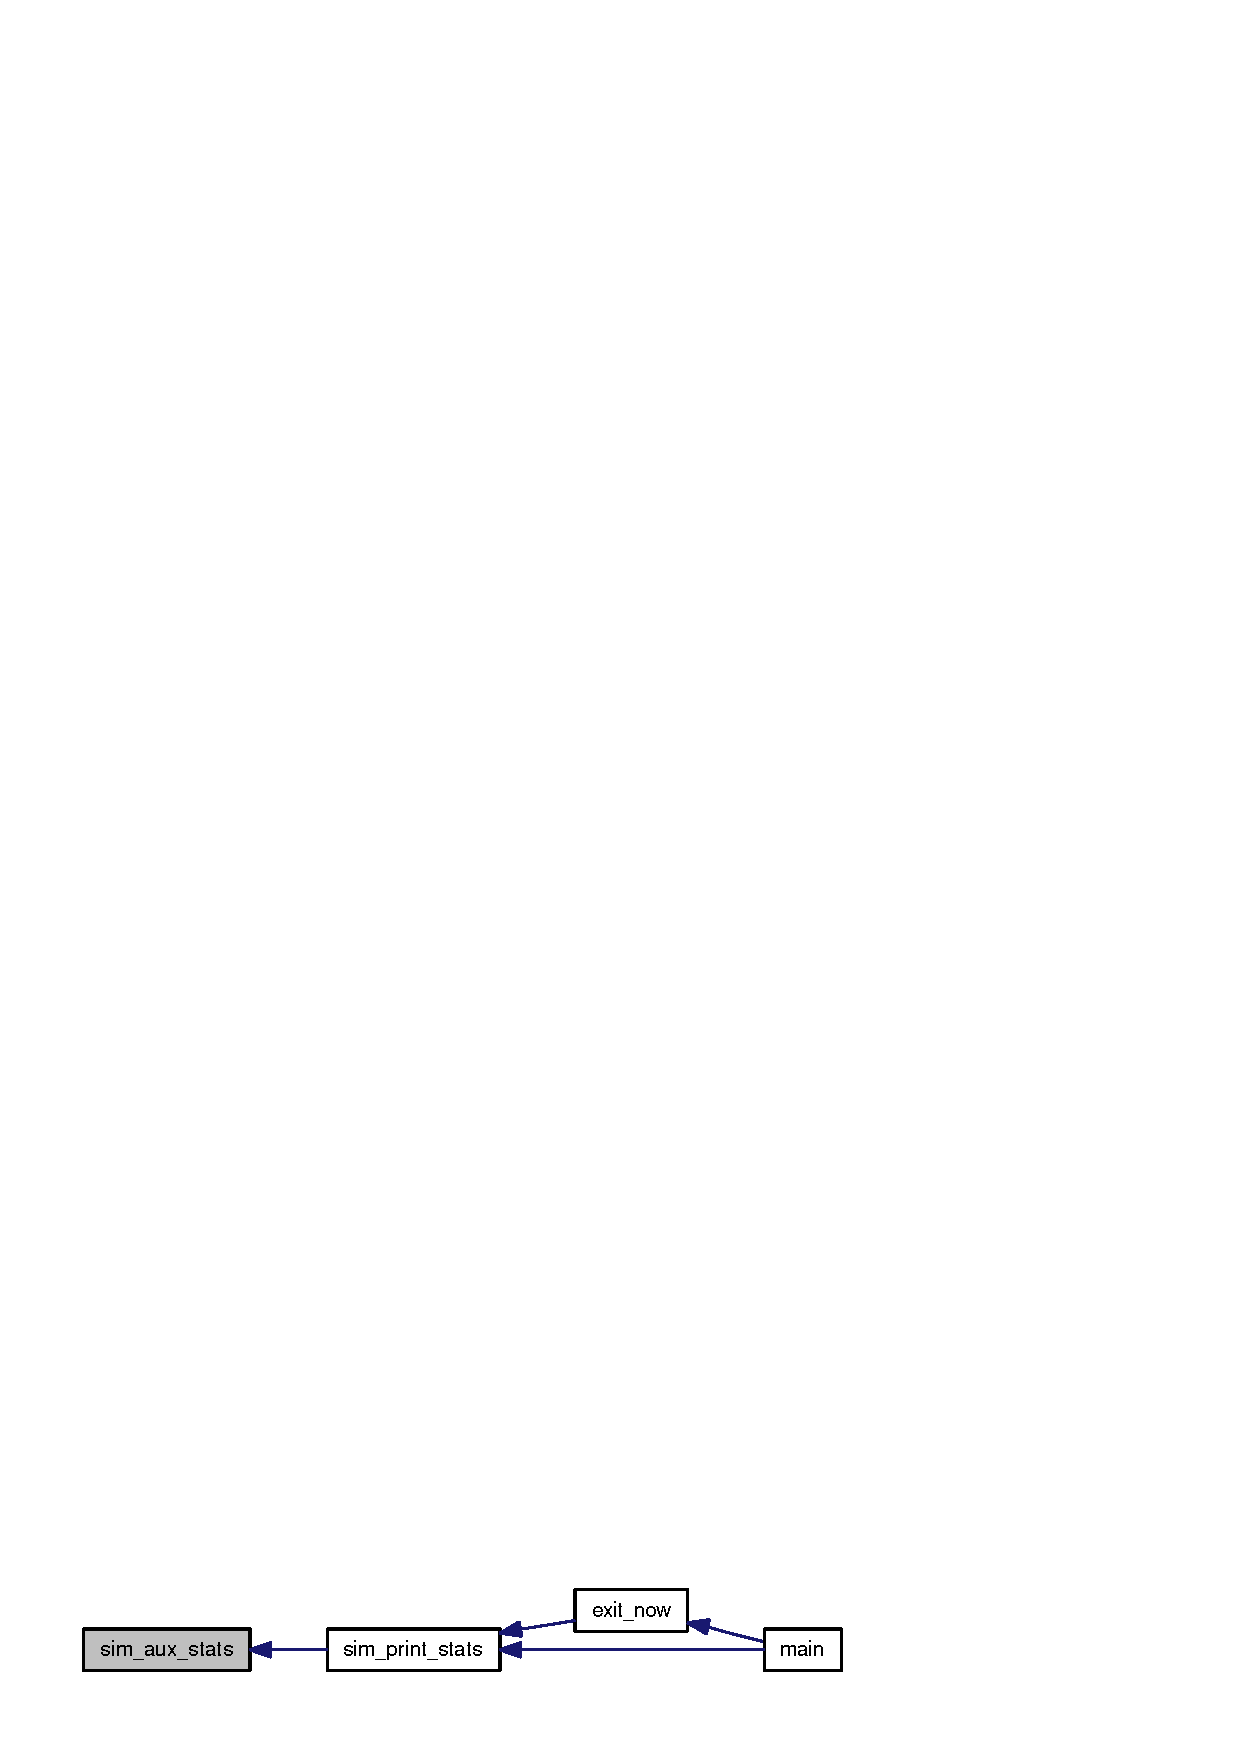
\includegraphics[width=204pt]{thread_8h_f0d3b44eaaad1fd53b38c9f82deb05fd_icgraph}
\end{center}
\end{figure}
\index{thread.h@{thread.h}!sim\_\-load\_\-prog@{sim\_\-load\_\-prog}}
\index{sim\_\-load\_\-prog@{sim\_\-load\_\-prog}!thread.h@{thread.h}}
\subsubsection[{sim\_\-load\_\-prog}]{\setlength{\rightskip}{0pt plus 5cm}int sim\_\-load\_\-prog (struct {\bf thread\_\-t} $\ast$ {\em thread}, \/  char $\ast$ {\em fname}, \/  int {\em argc}, \/  char $\ast$$\ast$ {\em argv}, \/  char $\ast$$\ast$ {\em envp})}\label{thread_8h_524226e93ca6adccd26acb04ba5f00e8}


\index{thread.h@{thread.h}!sim\_\-uninit@{sim\_\-uninit}}
\index{sim\_\-uninit@{sim\_\-uninit}!thread.h@{thread.h}}
\subsubsection[{sim\_\-uninit}]{\setlength{\rightskip}{0pt plus 5cm}void sim\_\-uninit (void)}\label{thread_8h_12f418d794abd0896d834c9582373b00}




Definition at line 437 of file sim-zesto.cpp.

Referenced by exit\_\-now().

Here is the caller graph for this function:\nopagebreak
\begin{figure}[H]
\begin{center}
\leavevmode
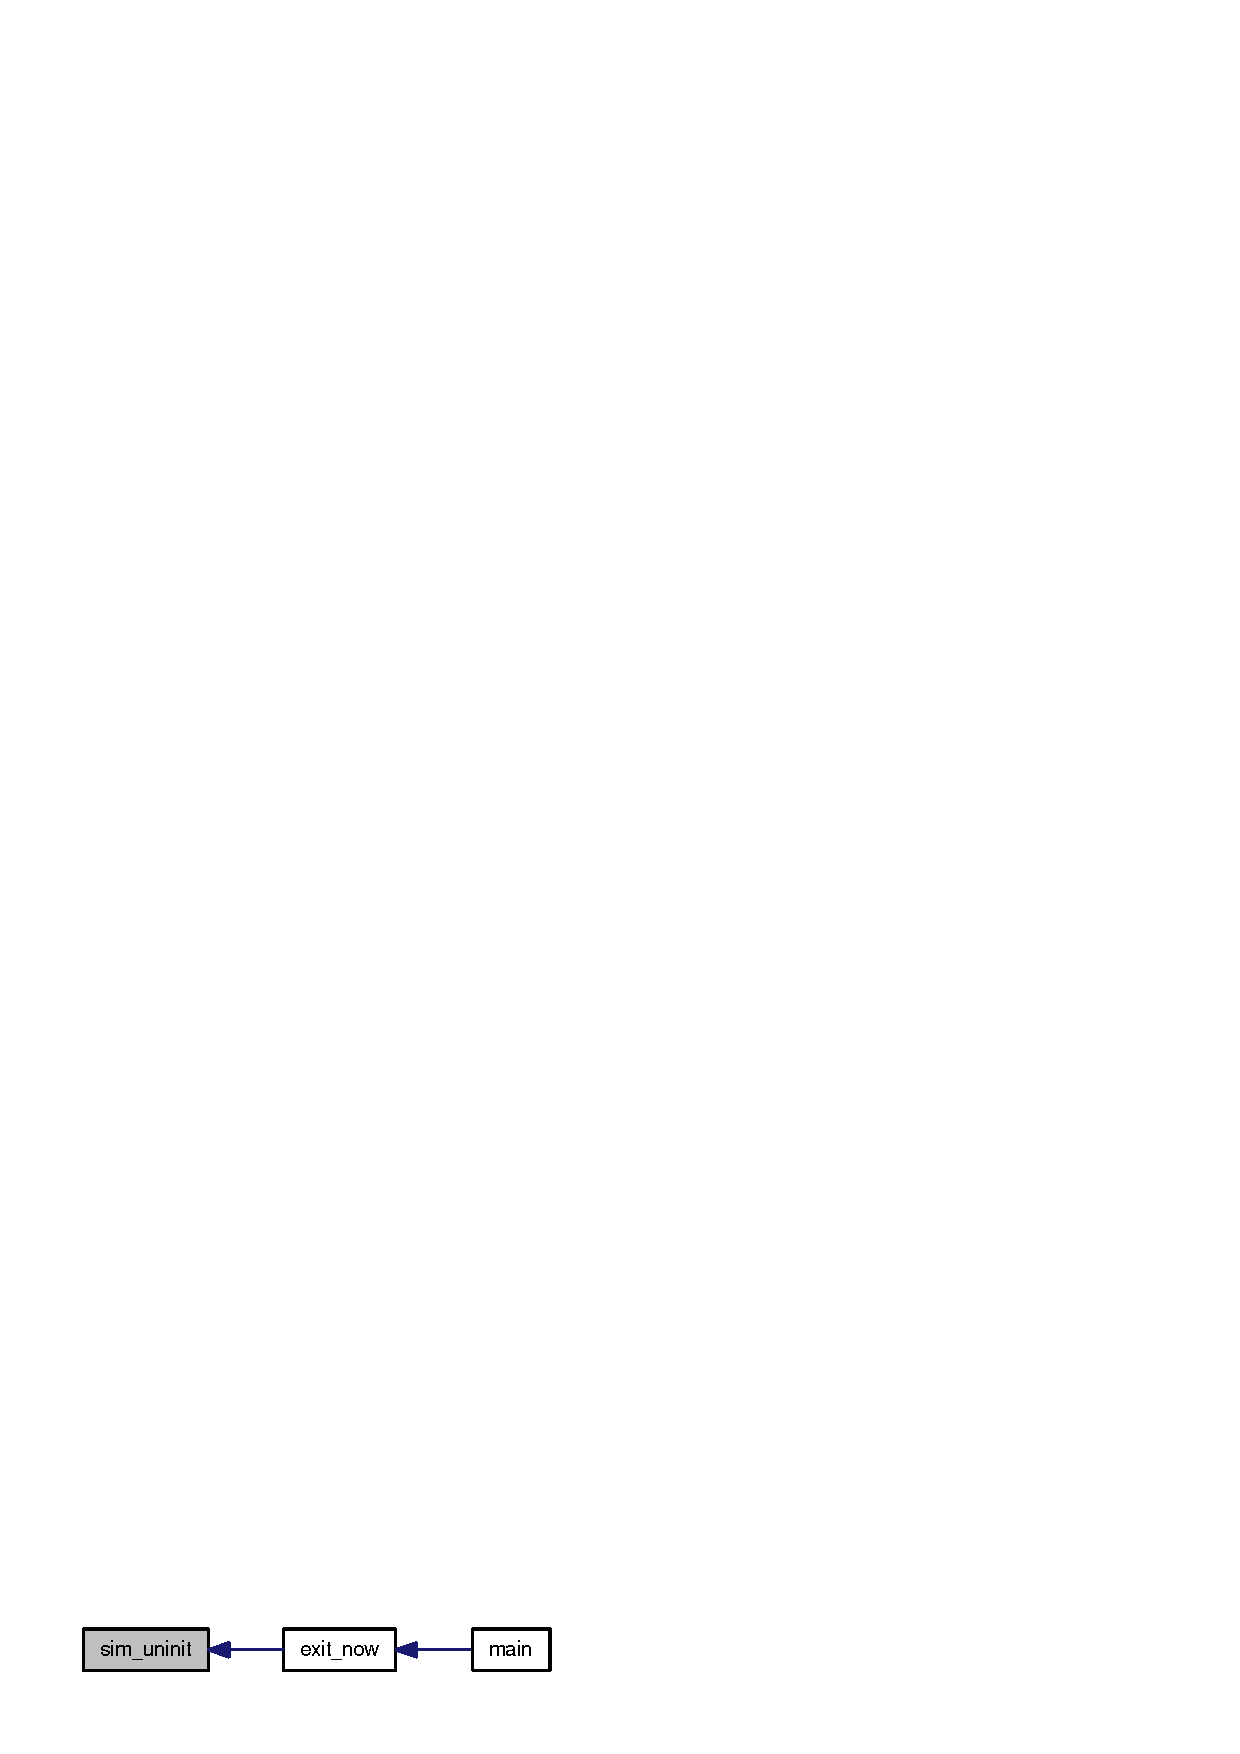
\includegraphics[width=134pt]{thread_8h_12f418d794abd0896d834c9582373b00_icgraph}
\end{center}
\end{figure}


\subsection{Variable Documentation}
\index{thread.h@{thread.h}!num\_\-threads@{num\_\-threads}}
\index{num\_\-threads@{num\_\-threads}!thread.h@{thread.h}}
\subsubsection[{num\_\-threads}]{\setlength{\rightskip}{0pt plus 5cm}unsigned int {\bf num\_\-threads}}\label{thread_8h_26a8352e9cd3bc9a6a35bc8d88152985}




Definition at line 186 of file sim-zesto.cpp.

Referenced by cache\_\-create(), cache\_\-create\_\-llc(), cache\_\-reset\_\-stats(), zesto\_\-component::downtick\_\-handler(), LLC\_\-reg\_\-stats(), main(), sim\_\-fastfwd(), sim\_\-main(), and sim\_\-post\_\-init().\index{thread.h@{thread.h}!simulated\_\-processes\_\-remaining@{simulated\_\-processes\_\-remaining}}
\index{simulated\_\-processes\_\-remaining@{simulated\_\-processes\_\-remaining}!thread.h@{thread.h}}
\subsubsection[{simulated\_\-processes\_\-remaining}]{\setlength{\rightskip}{0pt plus 5cm}int {\bf simulated\_\-processes\_\-remaining}}\label{thread_8h_1b2701dab57f1ffb6459bbde33452d68}




Definition at line 187 of file sim-zesto.cpp.

Referenced by core\_\-commit\_\-STM\_\-t::step(), and core\_\-commit\_\-DPM\_\-t::step().\index{thread.h@{thread.h}!threads@{threads}}
\index{threads@{threads}!thread.h@{thread.h}}
\subsubsection[{threads}]{\setlength{\rightskip}{0pt plus 5cm}struct {\bf thread\_\-t}$\ast$$\ast$ {\bf threads}}\label{thread_8h_f227be61b1f91b71aafae105501d92f7}




Definition at line 167 of file sim-zesto.cpp.

Referenced by main(), and core\_\-oracle\_\-t::syscall\_\-mem\_\-access().